% các thông số của văn bản
\setcounter{minitocdepth}{2}%*\label{line:lvSach_definition_setcounter}*)
\setcounter{secnumdepth}{3}
\renewcommand{\baselinestretch}{1.1}
\setlength{\parindent}{2 em}
\setlength{\parskip}{6pt}%*\label{line:lvSach_definition_setlength}*)

% xoá và xác lập lại tiêu đề chạy
\newcommand{\clearHeading}{
	\clearpage
	\pagestyle{empty}	      
	\cleardoublepage
	\pagestyle{fancyplain}
}

% định dạng trang
\pagestyle{fancyplain}%*\label{line:lvSach_definition_fancyplain}*)
\renewcommand{\chaptermark}[1]{%
	\markboth{\sl \chaptername~\thechapter.~#1}{}}
\renewcommand{\sectionmark}[1]{%
	\markright{\sl \thesection.~#1}}
 
 \fancyhf{}
 
\fancypagestyle{normalstyle}{% các chương%*\label{line:lvSach_definition_normalstyle}*)
  \lhead[\fancyplain{}{\thepage}]{\fancyplain{}{\rightmark}}
  \rhead[\fancyplain{}{\sl \leftmark}]{\fancyplain{}{\thepage}}
}

\makeatletter
\fancypagestyle{tocstyle}{% Mục lục
  \lhead[\fancyplain{}{\thepage}]{\fancyplain{}{\sl \contentsname}}
  \rhead[\fancyplain{}{\sl \@title}]{\fancyplain{}{\thepage}}
}

\fancypagestyle{nomenclstyle}{% Danh mục từ viết tắt
  \lhead[\fancyplain{}{\thepage}]{\fancyplain{}{\sl \nomname}}
  \rhead[\fancyplain{}{\sl \@title}]{\fancyplain{}{\thepage}}
}

\fancypagestyle{lofstyle}{% Danh mục các hình vẽ
  \lhead[\fancyplain{}{\thepage}]{\fancyplain{}{\sl \listfigurename}}
  \rhead[\fancyplain{}{\sl \@title}]{\fancyplain{}{\thepage}}
}

\fancypagestyle{lotstyle}{% Danh mục các bảng biểu
  \lhead[\fancyplain{}{\thepage}]{\fancyplain{}{\sl \listtablename}}
  \rhead[\fancyplain{}{\sl \@title}]{\fancyplain{}{\thepage}}
}

\fancypagestyle{indexstyle}{% Chỉ mục%*\label{line:lvSach_definition_indexstyle}*)
  \lhead[\fancyplain{}{\thepage}]{\fancyplain{}{\sl \indexname}}
  \rhead[\fancyplain{}{\sl \@title}]{\fancyplain{}{\thepage}}
}
\makeatother


% trang bìa chính
\makeatletter
\renewcommand{\maketitle}{%*\label{line:lvSach_definition_renewcommand_maketitle}*)
\begin{titlepage}%

\newgeometry{top=2cm, bottom=2cm, left=2cm, right=2cm}	%*\label{line:lvSach_definition_newgeometry}*)

\AddToShipoutPicture*{%
\begin{tikzpicture}
	\fill[color = yellow!30](0,0)rectangle(\paperwidth,\paperheight);%*\label{line:lvSach_definition_fill_yellow}*)
	\fill[color = red!50](0,0)rectangle(0.1\textwidth,\paperheight);%*\label{line:lvSach_definition_fill_red}*)
	\node at (0.5\paperwidth,0.35\textheight){ 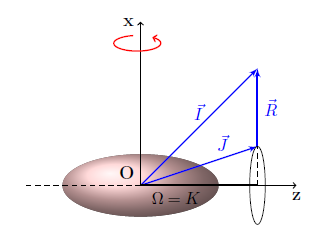
\includegraphics[width=0.5\textwidth] {figure/logo/couplage.png}};
\end{tikzpicture}
}      

\begin{center}

	\textbf{\Large \@author}
	\hrule
 	
	\vfill
		 	 
	{\fontsize{30}{36}\selectfont\textbf{\MakeUppercase \@title}}

	\vfill
	\vfill
	
	\begin{tikzpicture}
		\node(0,0){
\includegraphics[width=0.05\paperwidth] {figure/logo/logo_nxb} \MakeUppercase{ Nhà xuất bản Đại học quốc gia Hà Nội}};
	\end{tikzpicture}

 \end{center}
\end{titlepage}%
}%*\label{line:lvSach_definition_renewcommand_maketitle_end}*)
\makeatother



% trang bìa lót
\makeatletter
\newcommand{\maketitleBialot}{%*\label{line:lvSach_definition_bialot}*)
\begin{titlepage}%
	\hfill\bfseries\Large\MakeUppercase \@title
\end{titlepage}%
}
\makeatother

% trang bìa phụ
\makeatletter
\newcommand{\maketitleBiaphu}{
\begin{titlepage}%
	\centering
	{\bfseries\Large\@author}
	  \vfill
	{\bfseries\Huge\@title}
	    \vfill	
	\MakeUppercase{Nhà xuất bản Đại học quốc gia Hà Nội}
  \end{titlepage}
}%*\label{line:lvSach_definition_biaphu}*)
\makeatother


% thay đổi định dạng chương
% \p@ đơn vị 1pt, \z@ đơn vị 0pt
\makeatletter
\renewcommand{\@makechapterhead}[1]{%*\label{line:lvSach_definition_renewcommand_makechapterhead}*)
	{ \parindent \z@ \raggedleft 
	\vspace*{50\p@}%
	   	
	{\Huge\scshape \@chapapp~\thechapter}
	\vskip 20\p@
		    
	\hrule                                       
	\vskip 10\p@							
	\Huge \bfseries\scshape #1
	\vskip 20\p@						
	\hrule                                   
	    
	\vskip 50\p@	
	}
}

\renewcommand{\@makeschapterhead}[1]{
  {\parindent \z@ \raggedright
	\vspace*{50\p@}%
	
	\hrule                                       
	\vskip 10\p@%                   
	\Huge \bfseries\scshape #1
	\vskip 20\p@%                      
	\hrule                 
	                   
	\vskip 50\p@
	}
}%*\label{line:lvSach_definition_renewcommand_makechapterhead_end}*)
\makeatother


% định dạng lại mục lục
\makeatletter
\addtocontents{toc}{\hfill\textbf{Trang}\par}%*\label{line:lvSach_definition_dinhdangmucluc}*)
\titlecontents{chapter}
	[0cm]     
	{\addvspace{5pt}}  
	{\bf\scshape\@chapapp~\thecontentslabel\quad\\}
	{\bf\scshape} 										
	{\hfill\contentspage}

\g@addto@macro{\appendix}{
  \addtocontents{toc}{\protect\renewcommand*{\protect\@chapapp} {\protect\appendixname}}%
}%*\label{line:lvSach_definition_dinhdangmucluc_end}*)
\makeatother
